\chapter{Rozšíření pro Node-RED}
\label{ch:rozsireni}

Na základně poznatků z~kapitoly~\ref{sec:node-red-rozsireni} a navrženého komunikačního protokolu zde navrhnu a
zrealizuji vlastní rozšíření nástroje Node-RED -- předmětem budou detaily ze základní infrastruktury bloků a následně
příklady konkrétních aplikací přímo nasaditelných.
% \marginpar{\small Poznámky na okraji}

\section{Základní konfigurační blok}\label{sec:zakladni-konfiguracni-blok}
Základním stavebním prvkem pro další bloky je \ic{fis-node} (reprezentovaný třídou \mbox{\ic{FisNode})} -- využije se
tak
konfiguračních bloků, díky kterým nebude nutné přihlašovací údaje k~brokeru MQTT nebo identifikacím jednotlivých
uzlů zadávat více než jednou.

Jak uvádí dokumentace k~nástroji Node-RED~\cite{NodeRedDocs}, nedělitelnou součástí každého bloku v~Node-RED je jeho
konfigurační formulář pro editor.
Ten se skládá ze dvou povinných částí a jedné nepovinné -- z~povinných částí se jedná o~programovou definici pro
editor sítě v~jazyce Javascript a o~samotnou definici konfiguračního formuláře popsanou v~jazyce HTML.
Nepovinnou částí je poté uživatelská dokumentace dostupná přímo z~editoru.
Zkrácenou definici bloku pro editor lze vidět v~ukázce~\ref{code:fis-node-editor}, která kromě samotné registrace
obsahuje dva důležité aspekty.

Prvním je registrace do kategorie \ic{\'config\'}, což značí registraci konfiguračního bloku pro reprezentaci jednoho
IoT uzlu (uzel tedy nemá grafickou reprezentaci v~síti).
Druhým aspektem je výčet parametrů pro formulář, které následně bude možné použít pro samotné chování uzlu v~síti.
První parametr typu \ic{\'mqtt-broker\'} je určen pro konkrétní broker MQTT, pomocí kterého bude blok s~uzlem spojen
(jedná se o~konfigurační blok poskytnutý přímo nástrojem Node-RED).

Druhým parametrem je jednoznačná identifikace bloku, jejíž formát je omezen regulárním výrazem -- tento
parametr vychází ze zástupného symbolu \ic{NODE\_ID} z~navrženého protokolu popsaného
v~kapitole~\ref{sec:mqtt-kanaly}.
Tento symbol slouží pro odlišení jednotlivých uzlů, resp. konfiguračních bloků\footnote{Konkrétní tvar
identifikátoru (a jeho regulárního výrazu) není pro nástroj Node-RED podstatný, k~jeho upřesnění dojde až rámci
firmwaru uzlů popsaného v~kapitole~\ref{ch:firmware}.}.
Parametr \ic{nodeId} tedy následně bude použit pro sestavení kanálů MQTT pro odběr a publikaci zpráv.

% @formatter:off
\begin{code}[
    language=Javascript,
    label=code:fis-node-editor,
    caption={Registrace vlastního bloku do editoru sítě v~nástroji Node-RED -- kromě identifikačního klíče do
    registru bloků \ic{\'fis-node\'} se zde nachází definice parametrů a zařazení do konfiguračních bloků
    pomocí zvolené kategorie \ic{\'config\'}.}
]
RED.nodes.registerType('fis-node', {
    category: 'config',
    defaults: {
        broker: {type: "mqtt-broker", required: true, value: ""},
        nodeId: {
            value: "", required: true,
            validate: RED.validators.regex(/^[a-z0-9]{12}(*\textdollar*)/i)
        },
    },
    (*\ldots*)
});
\end{code}

V~ukázce~\ref{code:fis-node-constructor} je zobrazena část třídy \ic{FisNode}, reprezentující blok z~hlediska sítě.
V~konstruktoru této třídy dochází k~získání konfiguračních
parametrů z~formuláře, získání instance konfiguračního bloku pro připojení MQTT a přípravu kanálu na základě
\ic{NODE_ID}, resp. \ic{nodeId}.

Získaná instance bloku pro MQTT je zodpovědná za správu připojení -- není tedy nutné brát v~potaz možné odpojení a
nutnost znovupřipojení -- tato instance bude následně použita k~registraci odběrů a publikování zpráv do jednotlivých
MQTT kanálů protokolu.
Implementace tohoto bloku bohužel nemá dostupnou dokumentaci, veškeré poznatky o~jeho funkci jsou tedy brány přímo
z~jeho zdrojového kódu\footnote{\url{https://github
.com/node-red/node-red/blob/master/packages/node_modules/\%40node-red/nodes/core/io/10-mqtt.js}}.

% @formatter:off
\begin{code}[
    language=Javascript,
    label=code:fis-node-constructor,
    caption={Část konstruktoru třídy \ic{FisNode} obsluhující připojení brokeru MQTT a přípravu kanálů pro komunikaci.
    Důležitá je příprava části kanálů, které jsou následně použity pro publikování a odběr zpráv -- v~atributu
    \ic{_publish_topic} je uložen kanál s~identifikací uzlu, identifikace aplikace, dle kapitoly~\ref{sec:mqtt-kanaly}, připojí
    třída až při publikování pro konkrétní aplikaci. Druhým předpřipraveným kanálem je kanál pro odběr zprávy z~uzlu
    -- ten je uložen v~atributu \ic{_subscribe_topic}.}
]
class FisNode {
    constructor(config) {
        RED.nodes.createNode(this, config);
        this.broker = RED.nodes.getNode(config.broker);
        this.broker.connect(); // manually connect to MQTT broker
        // prepare topics for further usage
        this._publish_topic = ['fis', 'to', config.nodeId].join('/');
        this._subscribe_topic = ['fis', 'from', config.nodeId].join('/');
    }
    (*\ldots*)
    RED.nodes.registerType("fis-node", FisNode);
}
\end{code}
% @formatter:on

Implementace třídy \ic{FisNode} se vyznažuje několika dalšími vlastnostmi:
\begin{itemize}
    \item Signalizace stavu do editoru -- tato třída signalizuje skrz blok do editoru stav uzlu a konkrétní
    aplikace -- jak lze vidět na obrázku~\ref{fig:fis-node-status}, stav může nabývat tří hodnot:
    \begin{enumerate}
        \item uzel je online, aplikace je online -- vše v~pořádku, u~uzlu nedošlo k~odpojení či vypršení limitu pro
        odpověd dle parametru \uv{Keep Alive}, aplikace zasílá data
        \item uzel je online, aplikace offline -- uzel je připojen, avšak aplikace loguje zprávy na úrovni chyba
        \item uzel je offline -- u~uzlu došlo k~odpojení, buď vypnutím uzlu nebo chybou sítě (a vypršením limitu pro
        \uv{Keep Alive})
    \end{enumerate}
    \item Při smazání bloku dojde ke smazání aplikace -- instance třídy \ic{FisNode} je zaregistrovaná k~odběru
    události typu \ic{\'close\'} nad konkrétním blokem, čímž získá informaci od nástroje Node-RED, že došlo
k~odstranění bloku ze sítě.
    U~tohoto procesu je využit konfigurační kanál do uzlu společně s~resetováním parametru \uv{retain}, díky čemuž
    nedojde k~opětovnému zaslání konfigurace k~již neexistujícímu bloku.
    \item Fronta zpráv do brokeru -- třída je připravena i na stav, kdy dojde k~odpojení brokeru MQTT a bloky
    přesto chtějí komunikovat.
    Implementace toto řeší pomocí navázání funkcí na událost typu \ic{\'connect\'} nad
    objektem klienta MQTT spojení -- tyto funkce ve chvíli své invokace odešlou čekající zprávu a ukončí se.
    Toto chování je pro bloky zcela transparentní.
\end{itemize}

\begin{figure}
    \centering
    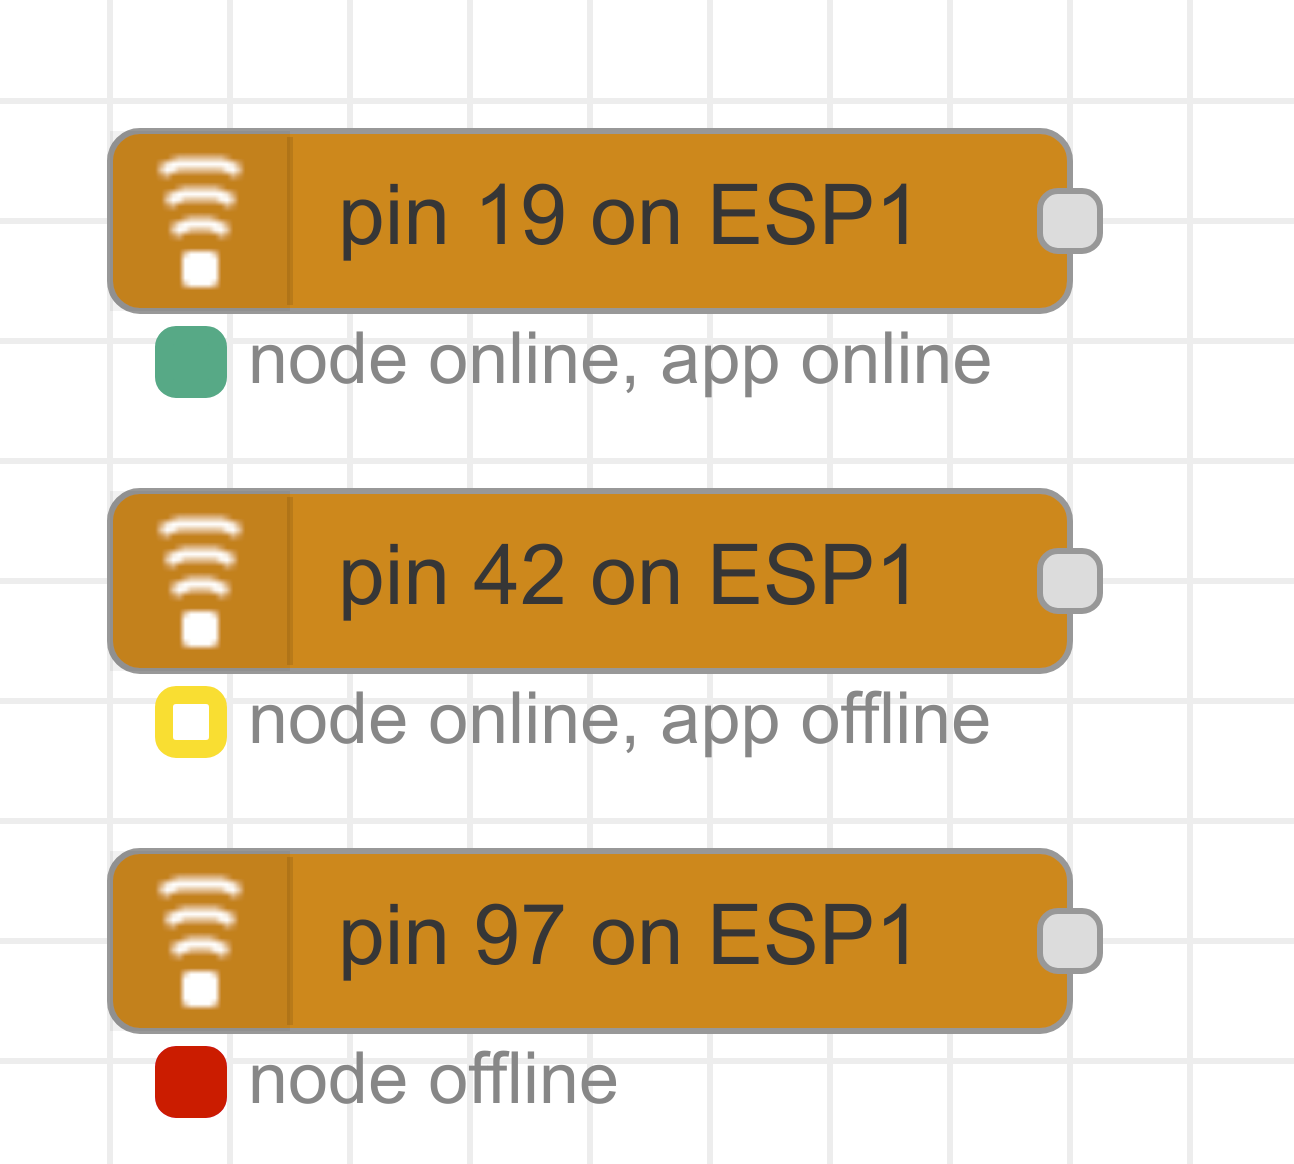
\includegraphics[width=.5\textwidth]{figures/fis-node-status.png}
    \caption{Výčet stavů bloku konkrétní aplikace -- třída \ic{FisNode} vyhodnocuje na základě dostupných informací
    (kanál pro logy, data a status uzlu) stav odpovídajícího uzlu a aplikace a tento stav signalizuje do editoru
    nástroje Node-RED. Konkrétně se jedná o~stav, kdy je vše v~pořádku, aplikace zasílá data (na obrázku první),
    stav, kdy je uzel připojen, avšak aplikace nezasílá či nepříjmá data (druhý případ) a poslední stav,
    kdy je uzel odpojen (třetí případ).}
    \label{fig:fis-node-status}
\end{figure}

Druhá povinná část, šablona konfiguračního formuláře do editoru, je úzce spjata s~registrací bloku -- jednotlivé
parametry zde musí odpovídat formulářovým prvkům, resp. jejich názvům, jak je uvedeno
v~ukázce~\ref{code:fis-node-template} -- kvůli funkci editoru, aby byl schopen učinit
formulář interaktivním a zároveň i srozumitelným pro jádro editoru a získávání hodnot z~něj.
V~ukázce lze také vidět speciální způsob definice HTML šablony -- šablona je obalena do elementu \ic{<script>} se
specifickou hodnotou v~atributu \ic{type="text/x-red"}\footnote{Standard HTML při tomto chování označuje
element \ic{<script>} jako \uv{data block} a prohlížeče jsou povinny obsah elementů s~tímto atributem dále
neinterpretovat.}.

% @formatter:off
\begin{code}[
    language=HTML,
    label=code:fis-node-template,
    caption={Ukázka z~implementace druhé povinné části deklarace bloku -- šablona formuláře v~jazyce HTML obsahuje
    jednotlivé vstupní pro pole pro korespondující parametry definovené v~registraci bloku do editoru
    v~ukázce~\ref{code:fis-node-constructor}.
    Atribut \ic{id="node-config-input-broker"} (a odpovídající) jsou důležité vzhledem k~chování editoru, nutná je shoda
    s~názvem parametru při registraci bloku -- stejně jako správné spárování šablony pomocí atributu
    \ic{data-template-name="fis-node"}.},
]
<script type="text/x-red" data-template-name="fis-node">
    <div class="form-row" id="node-config-row-broker">
        <label for="node-config-input-broker">MQTT</label>
        <input type="text" id="node-config-input-broker">
    </div>
    (*\ldots*)
    <div class="form-row">
        <label for="node-config-input-nodeId">Node ID</label>
        <input type="text" id="node-config-input-nodeId">
    </div>
</script>
\end{code}
% @formatter:on

Vzhledem k~aplikacím (a tedy již konkrétním blokům) poskytuje základní konfigurační blok několik metod pro práci
s~MQTT komunikací -- z~těch důležitějších se jedná o~\ic{appPublish} a \ic{appSubscribe}.
Prvně jmenovaná metoda, zobrazená v~ukázce~\ref{code:fis-node-app-publish}, slouží k~publikování zprávy pro
konkrétní aplikaci (vlastnost požadovaná v~kapitole~\ref{sec:pozadavky-na-protokol}) -- tedy do konkrétního kanálu.
Ten je v~tomto místě složen z~jednoznačné identifikace aplikace \ic{appId} (z~návrhu odpovídá symbolu \ic{APP_ID}) a
volitelně podkanálu -- použitá privátní metoda \ic{_publish} poté ke kanálu před odesláním zprávy připojí identifikaci
uzlu a dojde tak k~zacílení na konkrétní aplikaci na konkrétním uzlu.

% @formatter:off
\begin{code}[
    language=Javascript,
    label=code:fis-node-app-publish,
    caption={Detail z~implementace třídy \ic{FisNode} -- metoda \ic{appPublish} poskytuje možnost konkrétnímu bloku
    odeslání zprávy do odpovídající aplikace na uzlu, resp. do konkrétního subkanálu.}
]
appPublish(appId, payload, subtopic = null) {
    return this._publish(
        // subtopic is optional, filter() to avoid double slash in channel
        ['app', appId, subtopic].filter(_ => _).join('/'),
        {
            payload,
            qos: payload.qos,
            retain: payload.retain,
        }
    );
};
\end{code}
% @formatter:on

Posledním zmíněníhodným detailem implementace třídy \ic{FisNode} je metoda pro odběr zpráv z~aplikací na uzlech
\ic{appSubscribe}.
Tu mohou implementace jednotlivých bloků využít k~zaregistrování odběru konkrétního kanálu, resp. konkrétní aplikace
-- výsledný kanál je složen ze základního kanálu (pro směr do nástroje Node-RED sestaveného již v~konstruktoru),
identifikace aplikace \ic{appId} a volitelně podkanálu, opět dle navržené struktury protokolu z~kapitoly~\ref{sec:mqtt-kanaly}.
Uložená instance připojení k~brokeru MQTT poté slouží k~zaregistrování samotného odběru -- ten je realizován pomocí
funkce, kterou pro každou příchozí zprávu MQTT klient invokuje.
S~příchozími parametry je následně (po konverzi do formátu JSON) spuštěna funkce předaná při registraci konkrétního
odběru.

% @formatter:off
\begin{code}[
    language=Javascript,
    label=code:fis-node-app-subscribe,
    caption={Detail z~implementace třídy \ic{FisNode} -- metoda \ic{appSubscribe} je určená k~zaregistrování odběru
    kanálu odpovídajícího konkrétní aplikaci na konkrétním uzlu.
    Parametr \ic{qos} slouží k~nastavení konkrétní hodnoty QoS pro tento odběr, \ic{ref} je volitelná identifikace
    odběru, s~jejíž pomocí lze mazat konkrétní odběry.}
]
appSubscribe(appId, callback, subtopic = null, qos = 1, ref = 0) {
    const topic = [
        // subtopic is optional, filter() to avoid double slash in channel
        this._subscribe_topic, 'app', appId, subtopic
    ].filter(_ => _).join('/');
    return this.broker.subscribe(
        topic,
        qos,
        (topic, payload) => {
            callback(topic, JSON.parse(payload));
        },
        ref,
    );
};
\end{code}
% @formatter:on

\section{Implementace bloku pro vstupní aplikaci}\label{sec:implementace-bloku-pro-vstupni-aplikaci}
Blok pro vstupní aplikaci je z~pohledu nástroje Node-RED blokem, který do sítě produkuje zprávy (přijaté z~třetí
strany).
Funkce bloku reprezentující aplikaci na uzlu vychází ze základního konfiguračního bloku, který poskytuje podporu pro
komunikaci s~aplikací na uzlu, její konfiguraci, správu statusu bloku a další.
Konkrétní konfigurační blok (reprezentující fyzický uzel) nastaví uživatel v~editoru při konfiguraci bloku a nástroj
Node-RED poté instanci tohoto bloku (třídy \ic{FisNode}) zpřístupňuje pomocí utilitní funkce
\mbox{\ic{RED.nodes.getNode}} -- takto získaná instance tedy reprezentuje fyzický uzel skrz spojení MQTT.
V~ukázce~\ref{code:fis-dht-app} lze ve spodní části těla konstruktoru vidět dvě volání -- nad konfiguračním blokem se
prvně volá metoda \ic{config}.
Tato metoda zajišťuje napojení na servisní aplikaci určenou pro správu uzlu jako takového a dalších aplikací --
detaily její funkce budou popsány v~kapitole~\ref{sec:konfiguracni-aplikace}.
Volání konkrétně odešle do uzlu uživatelské nastavení společně s~identifikátorem aplikace \ic{\'dht-sensor\'} -- zahrnut
je typ senzoru a pin, na kterém je na uzlu připojen.
Pro konkrétní spárování dotčeného bloku s~aplikací na uzlu je odeslán i atribut bloku \ic{this.id}, který slouží
v~rámci nástroje Node-RED k~unikátní identifikaci uzlu v~celé síti\footnote{Atribut \ic{id} instancí bloků je
odsledován z~interní implementace běhového prostředí Node-RED -- \url{https://github
.com/node-red/node-red/blob/ed2a45e97551d9e43f079d69be8a490574e98559/packages/node_modules/\%40node-red/runtime/lib
/nodes/flows/Subflow.js}}, generován je náhodně implementací sítě.

Druhé volání je použití již popsané metody \ic{appSubscribe}, blok si zde registruje odběr dat přicházejících
z~uzlu.
Používá k~tomu vlastní atribut \ic{id}, kterým cílí na spárovanou aplikaci na uzlu, podkanál \ic{\'data\'}, který
následně použije i aplikace na uzlu, a funkci, pomocí které bude předávat příchozí zprávu z~uzlu, resp. brokeru MQTT,
do sítě nástroje Node-RED (skrz volání metody \ic{this.send}).

% @formatter:off
\begin{code}[
    language=Javascript,
    label=code:fis-dht-app,
    caption={Detail implementace vstupní aplikace (z~hlediska centrálního uzlu) -- jedná se o~aplikaci pro
    senzory měřící teplotu a vlhkost okolí.
    Konstruktor této třídy je zodpovědný za konfiguraci aplikace na uzlu za pomoci metody \ic{config} a následnou
    registraci odběru zprávy z~uzlu -- funkce volaná na příchozí zprávy z~nich přejímá data a zasílá je dále do sítě
    nástroje Node-RED (volání \ic{this.send})}.
]
class DhtSensor {
    constructor(config) {
        RED.nodes.createNode(this, config);
        this.fisNode = RED.nodes.getNode(config.node);

        // send app configuration to node
        this.fisNode.config('dht-sensor', this.id, {
            port: config.sensorPort,
            type: config.sensorType,
        });
        // subscribe data from node
        this.fisNode.appSubscribe(this.id, (topic, payload) => {
            this.send({
                temperature: payload.temperature,
                humidity: payload.humidity
            });
        }, 'data');
    }
}
\end{code}
% @formatter:on

\section{Implementace bloku pro výstupní aplikaci}\label{sec:implementace-bloku-pro-vystupni-aplikace}
Blok pro výstupní aplikaci je z~pohledu nástroje Node-RED blokem, který ze sítě konzumuje zprávy a zpracovává je dále.
V~ukázce~\ref{code:fis-node-neopixel-display} lze vidět implementaci bloku pro aplikaci ovládající bodový displej,
jejíž detaily budou popsány v~kapitole~\ref{subsec:implementace-vystupni-aplikace}.
Po standardním zavedení cílové aplikace na uzel si blok registruje odběr pomocí vlastní metody \ic{on} -- ta slouží
k~odběru příchozích zpráv do bloku, v~tomto případě převezme příchozí zprávu a zformátuje zprávu pro aplikaci
(kromě samotného textu k~zobrazení podporuje volitelně i požadovanou barvu).
Sestavená zpráva je odeslána pomocí \ic{appPublish} odpovídající aplikaci do subkanálu \ic{\'text\'}.

% @formatter:off
\begin{code}[
    language=Javascript,
    label=code:fis-node-neopixel-display,
    caption={Implementace bloku pro aplikaci ovládající bodový displej -- kromě samotné konfigurace na cílovém uzlu
    si uzel zaregistruje funkci pro odběr události typu \ic{\'input\'}.
    Událost tohoto typu notifikuje blok o~příchozí zprávě, která je v~tomto případě odeslána do aplikace k~zobrazení
    na displeji.}
]
class NeoPixelDisplay {
    constructor(config) {
        RED.nodes.createNode(this, config);
        this.fisNode = RED.nodes.getNode(config.node);
        // send app configuration to node
        this.fisNode.config('neopixel-display', this.id, {
            port: config.displayPort,
            width: config.width,
            height: config.height,
        });
        // send command to app on
        this.on('input', msg => {
            let payload = {text: msg.payload};

            if (msg.color)
                payload.color = msg.color;
            payload.retain = true;

            this.fisNode.appPublish(this.id, payload, 'text');
        });
    }
}
\end{code}
% @formatter:on

\section*{Použití v~dalších rozšířeních}\label{sec:pouziti-v-dalsich-rozsirenich}
Princip konfiguračních bloků reprezentující jednotlivé fyzické uzly je dobrým vstupním bodem pro další rozšíření --
ta lze realizovat pouze pomocí implementace bloku a příslušné aplikace.
Základem implementace bloku by byl již existující konfigurační blok poskytující komunikační a stavové rozhraní a
nutná implementace by byla pouze ta doménová, řešící konkrétní funkci bloku.
Na straně uzlu, resp. firmwaru, by se jednalo o~dvě části -- první částí by byla implementace ovladače konkrétní
periferie dle požadované funkce, druhou poté aplikace odpovídající bloku, která by měla ovladač na starost -- detaily
konkrétních principů firmwaru budou popsány v~kapitole~\ref{ch:firmware}.
Celé další rozšíření je možno realizovat externě k~existujícímu balíčku -- nástroj Node-RED
registruje typy konfiguračních bloků globálně, lze je tedy používat i mimo balíčky jejich definice (stejně jako je
použit blok pro
broker MQTT).